% id: 0183
% book: 쎈 중3-2 수학 · 02 삼각비의 활용
% section: 유형 03 실생활에서 직각삼각형의 변의 길이의 활용
% figure: crop:fig-0183.jpg
% answer: $67.5\,\mathrm{m}$
% answer_source: 답지
% variant_level: 0 (원본 전사)
% 이 파일은 build.mjs 가 items.json 에서 만든다. 고칠 때는 items.json 을 고친다.
\smash{\raisebox{1.5mm}{\dmkichul{쎈 중3-2 수학 0183번 · 38쪽}}}
\noindent\begin{minipage}[t]{0.58\linewidth}\vspace{0pt}\raggedright 현미가 오른쪽 그림과 같은 스키장의 슬로프를 따라 $\pt{A}$ 지점에서 $\pt{B}$ 지점까지 $150\,\mathrm{m}$를 내려갔을 때, 처음 위치의 높이에서 몇 $\mathrm{m}$ 낮아졌는지 구하시오. \cond{$\sin 27^\circ=0.45$로 계산한다.}\end{minipage}\hfill\begin{minipage}[t]{0.4\linewidth}\vspace{0pt}\centering 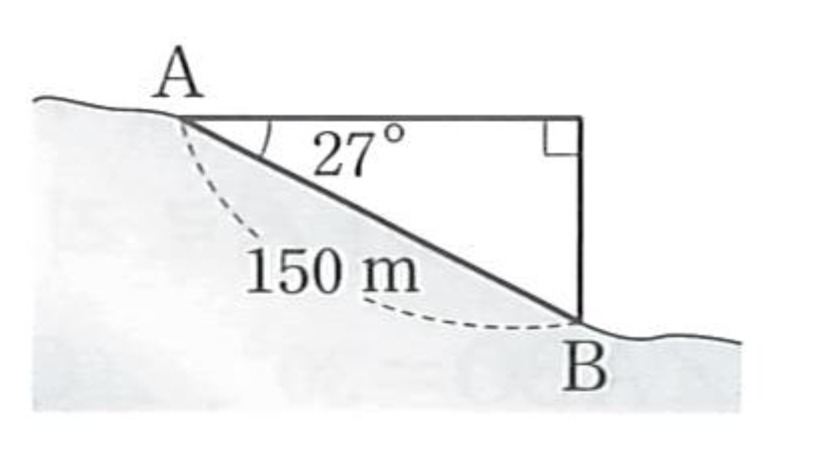
\includegraphics[width=97.9pt]{figures/fig-0183.jpg}\end{minipage}\par
